 \documentclass[a4paper, 12pt]{article}
\usepackage[mag=970]{newlistok}
%\usepackage{newlistok}
\usepackage{tikz}
%\usetikzlibrary{calc}

\renewcommand{\spacer}{\vfill}

\УвеличитьШирину{1.3truecm}
\УвеличитьВысоту{2.2truecm}

\newcommand{\ov}{\overline}
\newcommand{\Zm}[1]{\Z/ {#1}\Z}

\Заголовок{Классы вычетов}
\НомерЛистка{23}
\ДатаЛистка{19.09 -- 30.09.2018}
\Оценки{33/28/23}
\begin{document}


\СоздатьЗаголовок


\опр Пусть $m\in\N$.
%Напомним: говорят, что \выд{$a$ сравнимо с $b$ по модулю
%$m$}, если $a - b$ делится на~$m$. Обозначение: $a\equiv b
%\pmod{m}$.
Рассмотрим отношение эквивалентности <<разность делится на $m$>> на множестве целых чисел (см.~задачу 6, е листка 22), обозначение: $\equiv$.
Класс эквивалентности числа $r$ называют \выд{классом (вычетов) по модулю $m$} и обозначают $\ov{r}_m$ (или просто $\ov{r}$, если понятно, о каком $m$ идёт речь). Множество всех классов вычетов по модулю $m$ обозначают $\Zm{m}$. Класс $\ov{0}_m$ называют \выд{нулевым}. \копр

\задача \пункт Докажите, что $\ov{r}_m = \{mq + r\ |\ q\in\Z\}$. \пункт Сколько
элементов в множестве $\Zm{m}$? \кзадача

\опр
Для любых классов вычетов $\ov{r}$ и $\ov{s}$ по модулю $m$ определим
их {\it сумму}  и {\it произведение}, положив $\ov{r} + \ov{s} = \ov{r + s}$ и
$\ov{r}\cdot\ov{s} = \ov{r\cdot s}$.
\копр

\задача
Докажите, что сложение и умножение в $\Zm{m}$ не зависит от выбора представителей классов эквивалентности (то есть сложение и умножение {\it согласованы} с отношением эквивалентности). \кзадача

\УстановитьГраницы{0cm}{4.3truecm}
{\small
\noindent {\bf Замечание.} Можно представлять себе $\Zm{m}$ как множество
чисел $0$, $1$, $2$, \ldots, $m - 1$, которые складываются и
умножаются <<по модулю $m$>> (как остатки от деления на~$m$).
}


\пзадача
\пункт
Составьте таблицы сложения и умножения в $\Zm{2}$, $\Zm{3}$ и $\Zm{4}$.\\
\пункт
Найдите сумму всех элементов~$\Zm{m}$.
\кзадача

\пзадача
\onlyput{13.7truecm}{-1truecm}{%
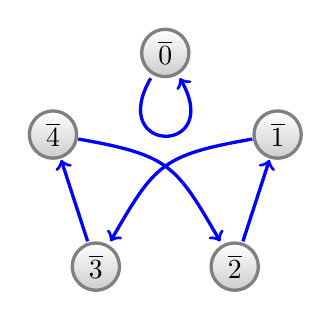
\begin{tikzpicture}[every node/.style={rectangle,minimum size=6mm,rounded corners=3mm,very thick,draw=black!50,top color=white,bottom color=black!20}]
  \node (A0) at (90:1.5) {$\ov{0}$};
  \node (A1) at (90-72:1.5) {$\ov{1}$};
  \node (A2) at (90-72*2:1.5) {$\ov{2}$};
  \node (A3) at (90+72*2:1.5) {$\ov{3}$};
  \node (A4) at (90+72:1.5) {$\ov{4}$};
  \draw[very thick,blue,->] (A0) .. controls +(-120:1.5) and +(-60:1.5) .. (A0);
  \draw[very thick,blue,->] (A2) -- (A1);
  \draw[very thick,blue,->] (A3) -- (A4);
  \draw[very thick,blue,->] (A4) .. controls +(-10:1.5) and +(120:1.5) .. (A2);
  \draw[very thick,blue,->] (A1) .. controls +(190:1.5) and +(60:1.5) .. (A3);
\end{tikzpicture}%
}
Изобразим элементы $\Zm{m}$ точками, зафиксируем %какой-либо
$\alpha\in\Zm{m}$ и из каждой точки $\omega$ провед\"ем стрелку в точку $\alpha\cdot \omega$.
Нарисуйте такие картинки для каждого $\alpha\in\Zm{m}$ при $m=6$ и $m=7$. (На рисунке --- пример для $\Zm{5}$, $\alpha=\ov{3}$.)
\кзадача



\ВосстановитьГраницы


\задача Приведите пример, когда произведение двух ненулевых классов
вычетов по модулю $m$ является нулевым классом. Такие классы
называют \выд{делителями нуля} в $\Zm{m}$. \кзадача

\пзадача Докажите, что натуральное число $m$ простое если и только если
в $\Zm{m}$ нет делителей нуля. \кзадача

\опр Класс $\beta\in\Zm{m}$ называется  \выд{обратным} (по умножению) к классу $\alpha\in\Zm{m}$, если $\alpha\cdot \beta = \ov{1}$.
Класс, к которому имеется обратный, называется \выд{обратимым} (по умножению).
\копр

{\small
\noindent {\bf Замечание.} Чтобы не писать всюду числа с чертой сверху, можно заменять классы на их представителей (числа без черты), но тогда равенства для классов надо заменять на соответствующие сравнения для их представителей: например, равенство $\ov{r}_m\cdot\ov{s}_m = \ov{1}_m$ эквивалентно сравнению $r\cdot s \equiv 1\!\pmod{m}$.
}

\пзадача  Выпишите все обратимые элементы и найдите к ним обратные в $\Zm{m}$ для $m=5,6,7,8$.
\кзадача

\задача
Докажите, что ненулевой класс не является делителем нуля если и только если он обратим.
\кзадача

\пзадача \пункт Докажите, что целое $m > 1$ простое если и только если
для любого ненулевого класса в $\Zm{m}$ найдётся обратный к нему класс из $\Zm{m}$.
\пункт Докажите, что обратный класс единствен.
\кзадача

\пзадача Решите уравнения %(то есть найдите все классы вычетов, для которых выполнено данное равенство):
\пункт $ 8x = 3$ в $\Zm{13}$; \пункт $7x = 2$ в $\Zm{11}$; \пункт $x^2=1$ в  $\Zm{6}$,  $\Zm{7}$,  $\Zm{8}$.
\кзадача


\задача
Для каких $\ov{a}$ из $\Zm{m}$ равенство $\ov{a}\cdot\ov{x}=\ov{a}\cdot\ov{y}$ при <<сокращении>> на $\ov{a}$ остаётся верным?
\кзадача


\задача\label{Z:Wils} %\сНовойСтроки
Пусть $p$ --- простое.
\пункт Найдите все такие $\alpha$ из $\Zm{p}$, что $\alpha^2=\ov{1}$
(то есть $\alpha$ обратен (по умножению) сам себе).
\пункт Докажите, что остальные элементы разбиваются на пары взаимнообратных.
\пункт\label{P:pr} Чему равно произведение всех ненулевых элементов $\Zm{p}$?
\пункт[Критерий Вильсона]
%\footnote\ov{1}{Александр Вильсон (1714 -- 1786) --- шотландский астроном и математик-любитель.}.)}
%профессор астрономии в Глазго.}.)}
Докажите, что целое число $m>1$ простое тогда и только тогда, когда $(m-1)!+1\equiv0\!\pmod{m}$.
\кзадача

\задача %{\it (Малая теорема Ферма)}
%\footnote[2]{Пьер Ферма (1602 -- 1665) --- великий французский математик, один из основоположников теории чисел.}.)}
Пусть $p$ --- простое, $\alpha\in\Zm{p}$, $\alpha\ne\ov{0}$.
\пункт
Домножим все элементы $\Zm{p}$ на $\alpha$. Докажите, что снова получатся
все элементы $\Zm{p}$.
\пункт
%Докажите, что $a^{p-1}\equiv1\!\pmod{p}$.
Выведите из пункта а) {\it малую теорему Ферма}: $\alpha^{p-1}=\ov{1}$.
%\пункт
%Докажите, что $b^{p}\equiv b\!\pmod{p}$ при любом целом $b$.
\кзадача

%\раздел{Многочлены}



\пзадача
\вСтрочку
\пункт
Пусть $p$ простое и имеет вид $4k+3$. Найдется ли такое целое $x$, что $x^2\equiv-1\!\pmod{p}$?\\
\пункт
Докажите, что если $x^2+1$ делится на неч\"етное простое число $p$,
то $p$ имеет вид $4k+1$.\\
\пункт
Докажите, что простых чисел вида $4k+1$ бесконечно много.\\
\пункт
Пусть $p$ простое и имеет вид $4k+1$. Найдите такое целое $x$, что $x^2\equiv-1\!\pmod{p}$.

\note{Указание.  Воспользуйтесь задачей \ref{Z:Wils}в).}
\кзадача

\задача Пусть $p$~--- простое. Докажите, что
\пункт $C_p^k$ делится на $p$ при всех таких целых $k$, что $1 < k < p$;\\
\пункт
в $\Zm{p}$ выполнено тождество $(\alpha + \beta)^p = \alpha^p + \beta^p$.
\пункт Выведите из пункта б) малую теорему Ферма.
\кзадача

%\раздел{Теорема Эйлера}

\пзадача
Изобразим элементы $\Zm{m}$ точками, зафиксируем
%%какой-либо
{\it обратимый (по умножению)} элемент\break $\alpha\in\Zm{m}$ и из каждой точки
$\omega\in\Zm{m}$ провед\"ем стрелку в точку $\alpha\cdot \omega$.
Докажите, что на этой картинке \\
\пункт движение по стрелкам распадается на непересекающиеся циклы;\\
\пункт каждый цикл, содержащий хоть один обратимый класс, весь состоит из обратимых классов;\\
\пункт циклы, состоящие из обратимых классов, имеют одинаковую~длину.
\кзадача



\задача {\it (Теорема Эйлера)}
%\footnote[3]{Леонард Эйлер (1707 -- 1783) --- швейцарец, работавший главным образом
%в России и в Германии. Крупнейший математик XVIII в., вн\"есший значительный
%вклад во все разделы математики.}.)}
Пусть $m\in\N$,
$\varphi(m)$ --- количество натуральных чисел, не превосходящих $m$ и взаимно
простых с $m$.  Докажите, что $a^{\varphi(m)}\equiv1\!\pmod{m}$,
если $a\in\Z$ и $(a,m)=1$.
\кзадача

%\задача Пусть $p_1,\dots,p_k$~--- различные простые, $\alpha_1,\dots,\alpha_k\in\N$. Найдите
%\пункт $\varphi({p_1}^{\alpha_1})$; \пункт $\varphi({p_1}^{\alpha_1})\dots\varphi({p_k}^{\alpha_k})$. \кзадача

\задача
Найдётся ли \пункт $3^k$, оканчивающееся на 0001;
\пункт $2^k-1$, делящееся на данное нечётное~$x$?
%Докажите, что для нечётного $m$\пункт найдётся такое $n$, что $2^n-1\del m$; \пункт $2^{m!}-1\del m$.
\кзадача

\ЛичныйКондуит{0mm}{6mm}
% \GenXMLW
%\СделатьКондуит{5.4mm}{7mm}

\end{document}
